\chapter{Synthèse d'une régulation de position par PID}

La synthèse d'une régulation de position par un régulateur PID a été envisagée. L'objectif de cette démarche est d'obtenir un système dont les composants sont connus et dont l'étude s'avère plus simple qu'une approche par retour d'état. Une fois un comportement satisfaisant obtenu, une analyse des pôles sera réalisée afin de pouvoir effectuer un placement de pôles au sein de la régulation d'état.\\

La synthèse s'appuie sur le schéma bloc présenté dans la \autoref{fig:PIDBloc} :

\begin{figure}[H]
    \centering
    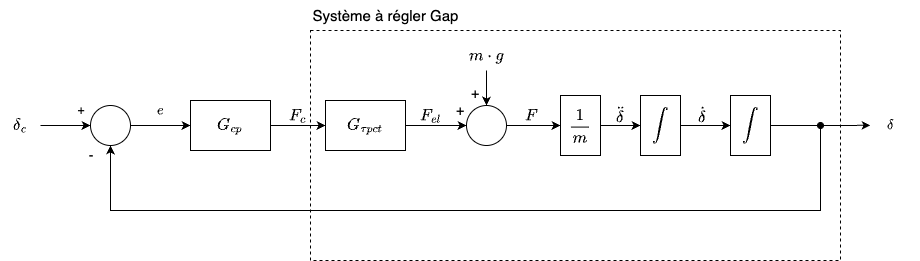
\includegraphics[width=1\linewidth]{assets/appendix/08-PID/PIDBloc.png}
    \caption{Schéma bloc de la régulation de position par PID}
    \label{fig:PIDBloc}
\end{figure}

À l'instar de la régulation d'état, l'ensemble des retards a été regroupé au sein d'un bloc unique.

Le système à régler est alors défini par l'\autoref{eq:Gap} :

\begin{equation}
    G_{ap} = G_{pct}\cdot \frac{1}{m\cdot s^2}
    \label{eq:Gap}
\end{equation}

Le diagramme de Bode du système à régler est représenté sur la \autoref{fig:BodeGap} :

\begin{figure}[H]
    \centering
    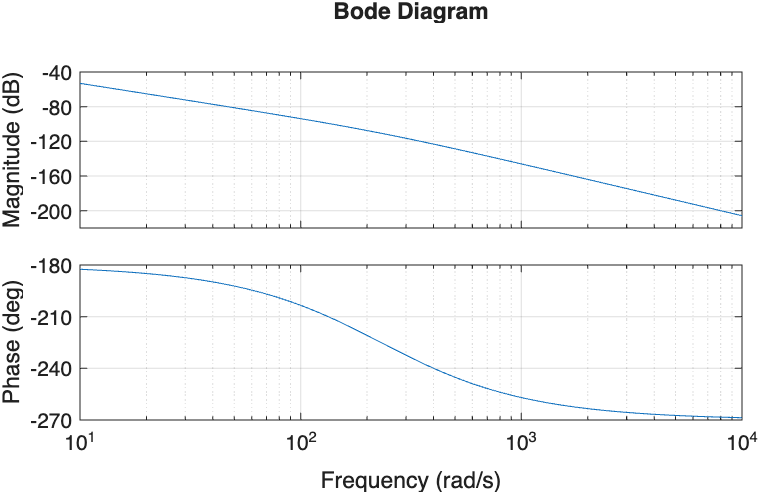
\includegraphics[width=1\linewidth]{assets/appendix/08-PID/BodeGap.png}
    \caption{Diagramme de Bode du système à régler $G_{ap}$}
    \label{fig:BodeGap}
\end{figure}

La fonction de transfert du régulateur $G_{cp}$ se définit comme celle d'un PID, exprimée par l'\autoref{eq:Gcp} :

\begin{equation}
    G_{cp} = K_{pid}\cdot\frac{1 + \tau_i \cdot s + \tau_i \cdot\tau_d\cdot s^2}{\tau_i \cdot s}
    \label{eq:Gcp}
\end{equation}

La synthèse se concentre dès lors sur la détermination des paramètres $K_{pid}$, $\tau_i$ et $\tau_d$.\\

Afin de simplifier cette recherche, le critère de l'optimum symétrique a été employé. La constante de temps de l'action intégrale $\tau_i$ est ainsi fixée à quatre fois la valeur de la constante de temps de l'action dérivée $\tau_d$, comme formulé dans l'\autoref{eq:OptSym} :

\begin{equation}
    \tau_i = 4\cdot\tau_d
    \label{eq:OptSym}
\end{equation}

Cette méthode permet de réduire l'étude à deux paramètres inconnus : la valeur de $\tau_d$ dans un premier temps, puis le gain $K_{pid}$.\\

La grandeur $\tau_d$ est définie comme le produit de la somme des petites constantes de temps par un coefficient $N$, selon l'\autoref{eq:TauD} :

\begin{equation}
    \tau_d = N\cdot\sum\tau_{pct} = N\cdot 4.27\cdot 10^{-3}
    \label{eq:TauD}
\end{equation}

À l'image de la synthèse de la régulation de courant, une analyse paramétrique a été menée pour des valeurs de $N$ comprises entre 1 et 20. À l'issue de ces simulations, l'évolution de la bande passante et de l'erreur a été évaluée en fonction de $N$. Seules les configurations garantissant une marge de phase de 45° ont été retenues. Le choix final du paramètre $N$ repose sur un compromis optimal entre la largeur de la bande passante et la prédiction de l'erreur.

Le tracé pour différentes valeurs de $N$ est disponible sur la \autoref{fig:ChoixNPID} :

\begin{figure}[H]
    \centering
    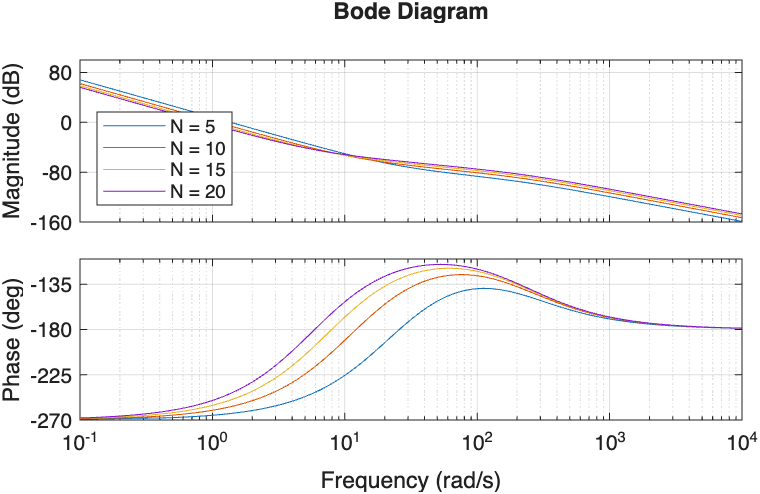
\includegraphics[width=1\linewidth]{assets/appendix/08-PID/ChoixN.png}
    \caption{Diagramme de Bode pour différentes valeurs de $N$}
    \label{fig:ChoixNPID}
\end{figure}

La bande passante est illustrée par la \autoref{fig:BPPID} :

\begin{figure}[H]
    \centering
    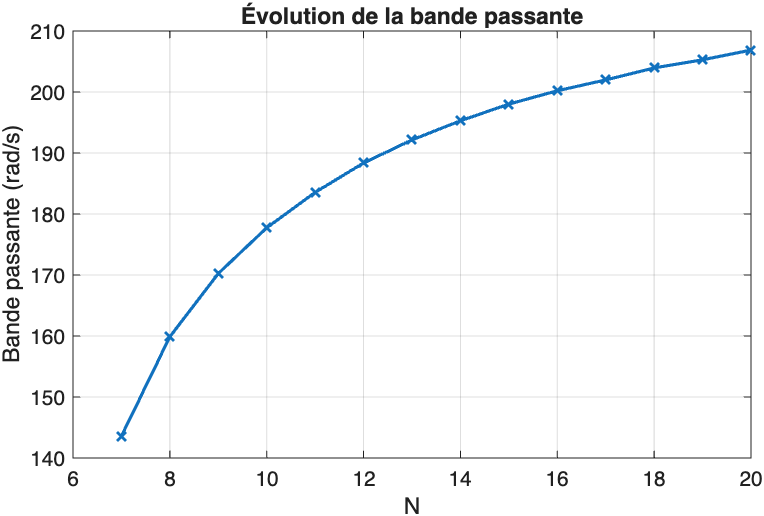
\includegraphics[width=1\linewidth]{assets/appendix/08-PID/BP.png}
    \caption{Évolution de la bande passante en fonction de $N$}
    \label{fig:BPPID}
\end{figure}

Le calcul de l'erreur est réalisé en intégrant l'erreur lors d'un essai en régulation de maintien, ce qui correspond à la surface comprise entre la consigne et la réponse du système. L'évolution de cette surface en fonction de $N$ est présentée sur la \autoref{fig:ErrorPID} :

\begin{figure}[H]
    \centering
    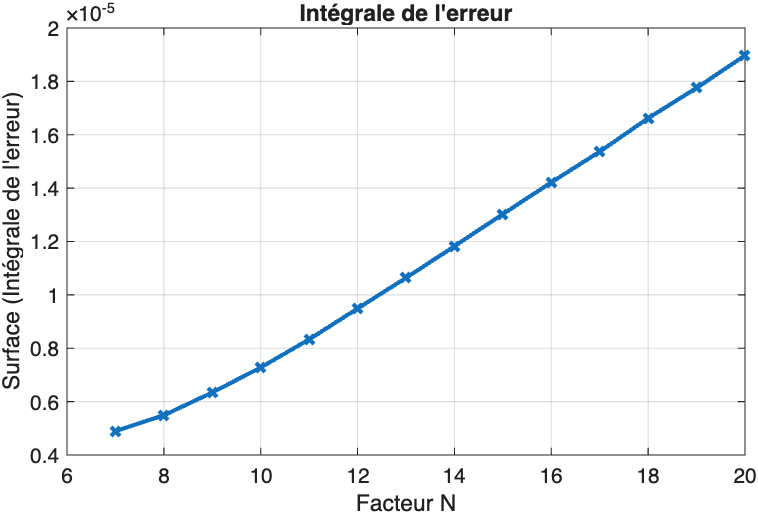
\includegraphics[width=1\linewidth]{assets/appendix/08-PID/Erreur.png}
    \caption{Évolution de l'erreur en fonction de $N$}
    \label{fig:ErrorPID}
\end{figure}

Le choix s'est porté sur la valeur $N=12$, offrant un équilibre satisfaisant entre la bande passante et l'erreur.

Il est alors possible de déterminer le gain $K_{pid}$ en recherchant, pour cette valeur de $N$, le gain assurant une marge de phase de 45° :

\begin{figure}[H]
    \centering
    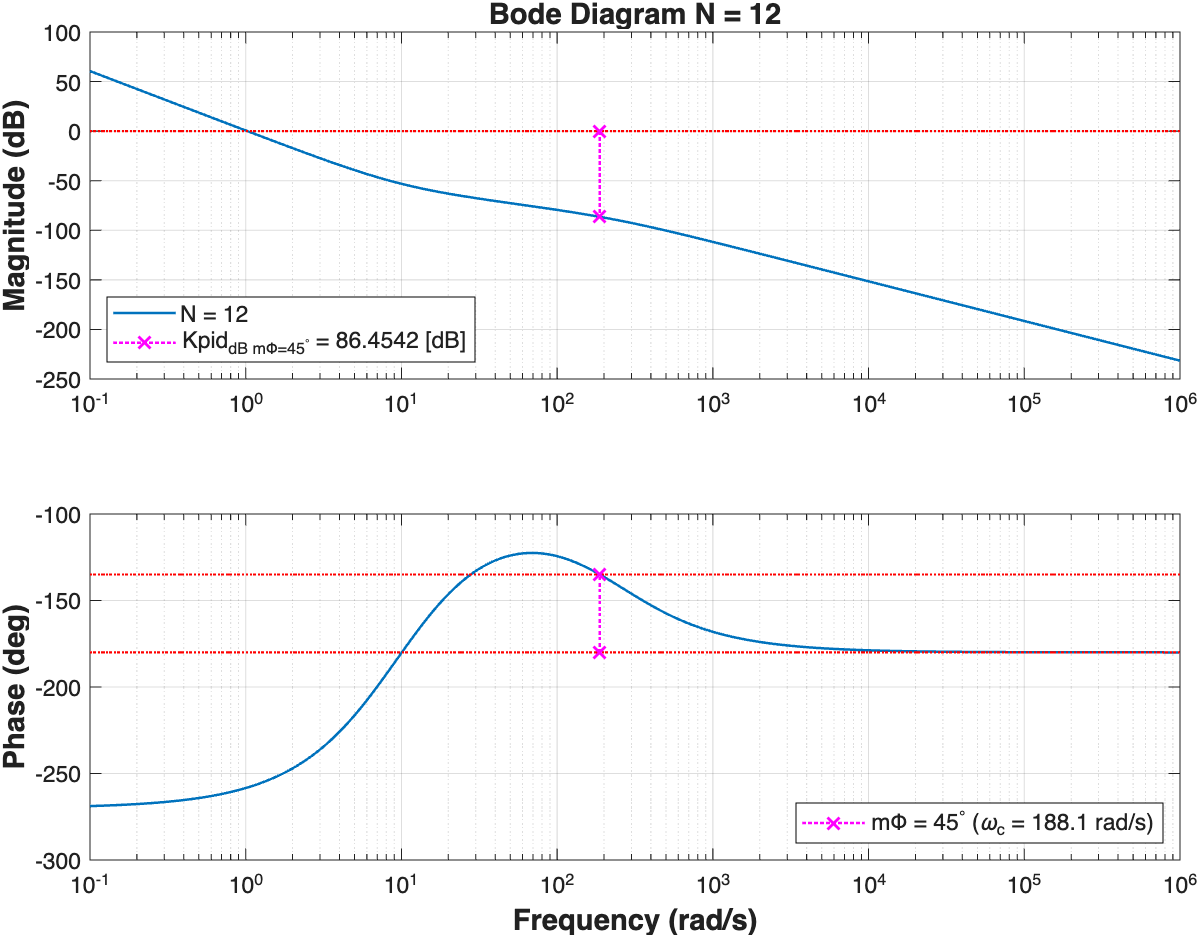
\includegraphics[width=1\linewidth]{assets/appendix/08-PID/RechercheKpid.png}
    \caption{Détermination du gain $K_{pid}$}
\end{figure}

Cette configuration détermine les paramètres finaux du régulateur PID, présentés dans l'\autoref{eq:ParamPID} :

\begin{equation}
    K_{pid} = 20889 \quad \tau_i = 207.7 \text{ ms} \quad \tau_d = 51.9 \text{ ms}
    \label{eq:ParamPID}
\end{equation}

Le diagramme de Bode en boucle ouverte est visible sur la \autoref{fig:BOPID} :

\begin{figure}[H]
    \centering
    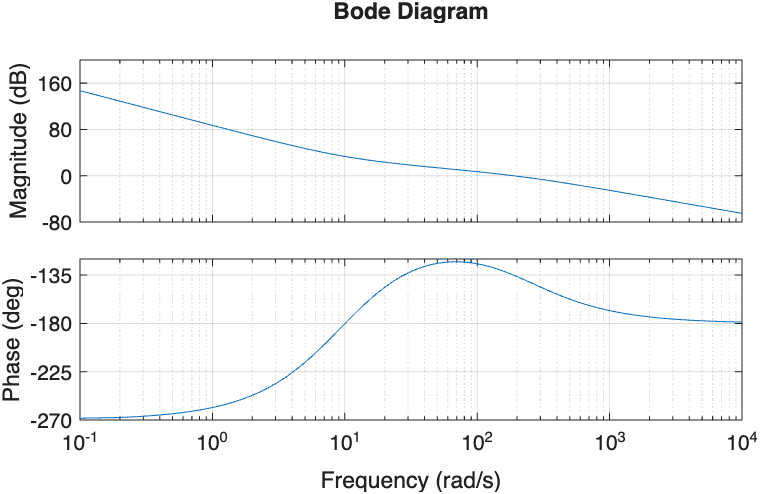
\includegraphics[width=1\linewidth]{assets/appendix/08-PID/Gbo.png}
    \caption{Diagramme de Bode de la boucle ouverte}
    \label{fig:BOPID}
\end{figure}

Afin de vérifier le comportement du système, un saut unitaire en boucle fermée a été réalisé. Les résultats sont présentés sur le tracé de la \autoref{fig:RepIndPID} :

\begin{figure}[H]
    \centering
    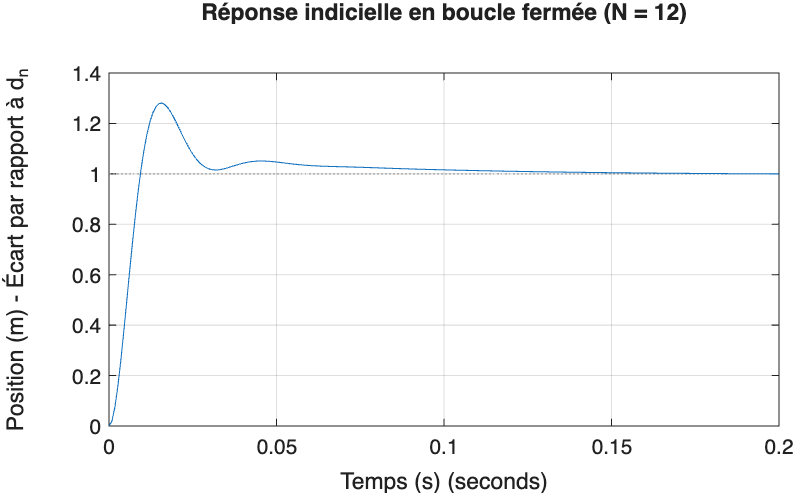
\includegraphics[width=1\linewidth]{assets/appendix/08-PID/RepIndi.png}
    \caption{Réponse indicielle du système en boucle fermée}
    \label{fig:RepIndPID}
\end{figure}

Cette réponse indicielle confirme la réactivité adéquate du système vis-à-vis de la maquette.

Cette étude nécessite toutefois d'être validée par des essais physiques sur le démonstrateur, la régulation n'étant pour l'instant qu'au stade de la modélisation.